Recurrent neural networks, or RNNs for short, are essentially multiple neural networks that feed into each other a specified number of times \citep{rumelhart1986learning}. Similar to traditional neural networks, these networks have an input layer, a hidden state, and an output layer. As recurrent patterns can be difficult to visualize, these networks are often visualize in an "unrolled" state. This is visualized in Figure \ref{fig:RNN}, where instead of the network looping back into itself 3 times, the 3 different time states are visualized as separate networks.

\begin{figure}[ht]
    \centering
    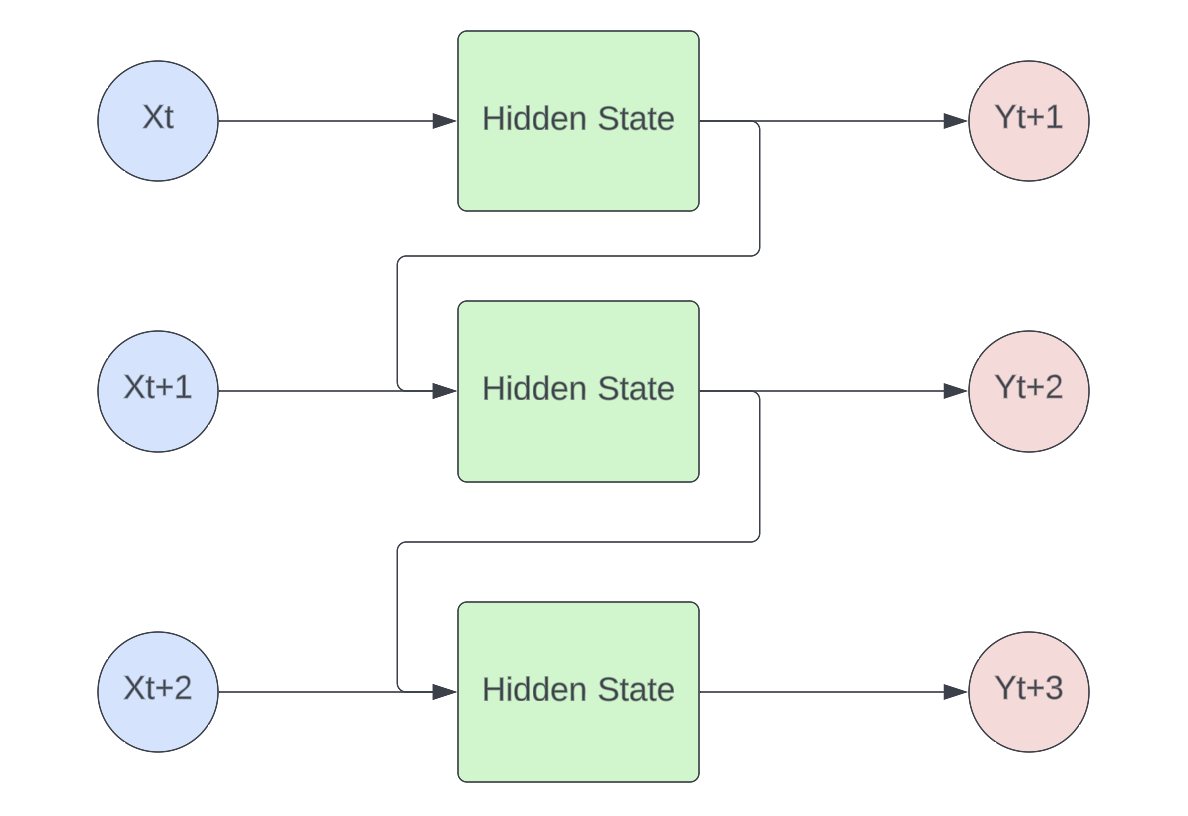
\includegraphics[width=0.6\linewidth]{"Figures/Recurrent_NN.png"}
    \caption{A visualization of an "unrolled" recurrent neural network. This specific example uses 3 time-points of information to get a prediction.}
    \label{fig:RNN}
\end{figure}

Recurrent neural networks are very useful when working with time series as observations depend on previous observations. A key issue that can arise when using too many time points to predict a single output is an exploding/vanishing gradient, which occurs when a weight associated with time point 1 ends up being multiplied by itself \textit{n} times to predict \textit{n} time points ahead. Using Figure \ref{fig:RNN} as an example network, the prediction for $Y_{t+1}$ would look like:
\begin{equation*}
    y_1 = \sigma[w_1\cdot x_1 + b_1]\cdot w_2 + b_2
\end{equation*}
Then, using that prediction in the following time points prediction:
\begin{equation*}
    y_2 = \sigma[w_1\cdot x_2 + w_3\cdot\sigma[w_1\cdot x_1 + b_1] + b_1]\cdot w_2 + b_2
\end{equation*}
Similarly, for the final prediction:
\begin{equation*}
    y_3 = \sigma[w_1\cdot x_3 + w_3\cdot \sigma[w_1\cdot x_2 + w_3\cdot\sigma[w_1\cdot x_1 + b_1] + b_1] + b_1]\cdot w_2 + b_2
\end{equation*}
In the equations above, $w_1$ represents the weight applied to the input, $w_2$ represents the weight applied to the output of the hidden state, and $w_3$ represents the weight applied to past predictions in the current prediction. Similarly, $b_1$ represents the bias being added to the input and $b_2$ represents the bias added to the hidden layer's output. If $w_3$ is a value above 1, this causes the value of $x_1$ to have a much larger impact on the final prediction than other inputs. To solve this, "memory" can be added to recurrent neural networks.